
\documentclass[a3paper,12pt]{article} % Specify A3 paper size and font size
\usepackage{amsmath}
\usepackage{amssymb} % Include this package for \mathbb
\usepackage[margin=1in]{geometry} % Adjust the margin as needed
\usepackage{graphicx} % Include this package for \includegraphics

\begin{document}

\author{kipngeno koech - bkoech}
\title{Homework 6 - Mathetmatical Foundations of Machine Learning Engineers}
\maketitle

\medskip


\subsection*{1. Entropy of a Bernoulli Random Variable [10 points] } 

Consider a random variable $X$ that follows a Bernoulli distribution $B(1, p)$ with $0 < p < 1$. We define the entropy of $X$ as 
\[
H(p) = \mathbb{E}[-\log(p(X))].
\]
(You will need to read a little bit about entropy or consult a TA during office hours.)

\begin{enumerate}
    \item[(a)] Derive the second derivative $H''(p)$ of $H(p)$. If $H''(p) \leq 0$, $H(p)$ is called concave. Is $H(p)$ a concave function of $p$? \hfill (5 points)
    
    The probability mass function of a Bernoulli random variable is given by:
    \[
    p(x) = \begin{cases}
    p & \text{if } x = 1, \\
    1 - p & \text{if } x = 0.
    \end{cases}
    \]
    The expected value is given by:
    \[
    \mathbb{E}[X] = \sum_{x \in \{0, 1\}} x \cdot p(x).
    \]
    so the entropy of $X$ is:
    \[
    H(p) = -\sum_{x \in \{0, 1\}} p(x) \log(p(x)).
    \]
    this is equivalent to:
    \[
    H(p) = -p \log(p) - (1 - p) \log(1 - p).
    \]
    The first derivative of $H(p)$ with respect to $p$ is:
    \[
    H'(p) = -\log(p) - 1 + \log(1 - p).
    \]
    The second derivative of $H(p)$ with respect to $p$ is:
    \[
    H''(p) = -\frac{1}{p} - \frac{1}{1 - p}.
    \]
    The second derivative is always negative for $0 < p < 1$, so $H(p)$ is a concave function of $p$.
    \\ This means that the entropy of a Bernoulli random variable is a concave function of the probability $p$.
    \item[(b)] Find the value of $p \in (0, 1)$ that maximizes $H(p)$. \hfill (5 points)
    To maximize $H(p)$, we set the first derivative to zero:
    \[
    H'(p) = -\log(p) - 1 + \log(1 - p) = 0.
    \]
    \[
    \log(1 - p) - \log(p) = 1.
    \]
    \[
    \log\left(\frac{1 - p}{p}\right) = 1.
    \]
    \[
    {1 - p} = p
    \]
    \[
    p = \frac{1}{2}.
    \]
\end{enumerate}

\vspace{30pt}
\subsection*{2. Binary Classification with Logistic Regression [70 points]} 

Consider a binary classification problem where $y \in \{0, 1\}$ and $\mathbf{x} \in \mathbb{R}^2$. Our goal is to model $p(y = 1 \mid \mathbf{x})$. We decide to use a Bernoulli distribution parameterized by the random vector $\mathbf{w} \in \mathbb{R}^2$, such that:
\[
p_{\text{model}}(y = 1 \mid \mathbf{x}; \mathbf{w}) = \sigma(\mathbf{w}^\top \mathbf{x}),
\]
\[
p_{\text{model}}(y = 0 \mid \mathbf{x}; \mathbf{w}) = 1 - \sigma(\mathbf{w}^\top \mathbf{x}),
\]
where $\sigma(z) = \frac{1}{1 + e^{-z}}$ is the sigmoid function.

(a) Show that
\[
p_{\text{model}}(y \mid \mathbf{x}; \mathbf{w}) = \big(\sigma(\mathbf{w}^\top \mathbf{x})\big)^y \big(1 - \sigma(\mathbf{w}^\top \mathbf{x})\big)^{1-y}.
\]
\hfill (5 points)

The probability mass function of a Bernoulli random variable is given by:
\[
p(y \mid \mathbf{x}; \mathbf{w}) = \begin{cases}
\sigma(\mathbf{w}^\top \mathbf{x}) & \text{if } y = 1, \\
1 - \sigma(\mathbf{w}^\top \mathbf{x}) & \text{if } y = 0.
\end{cases}
\]
This is equivalent to:

\[
p(y \mid \mathbf{x}; \mathbf{w}) = \big(\sigma(\mathbf{w}^\top \mathbf{x})\big)^y \big(1 - \sigma(\mathbf{w}^\top \mathbf{x})\big)^{1-y}.
\]
This is because:
\[
\sigma(\mathbf{w}^\top \mathbf{x})^1 = \sigma(\mathbf{w}^\top \mathbf{x}), \quad \sigma(\mathbf{w}^\top \mathbf{x})^0 = 1 - \sigma(\mathbf{w}^\top \mathbf{x}).
\]

(b)
Table 1 contains 10 samples, $(\mathbf{x}, y)$, obtained from the data-generating distribution $p_{\text{data}}$. The KL divergence between $p_{\text{data}}$ and $p_{\text{model}}$ is given as:
\[
D_{\text{KL}}(p_{\text{data}} \mid\mid p_{\text{model}}) = \mathbb{E}_{\mathbf{x}, y \sim p_{\text{data}}} \big[\log p_{\text{data}}(y \mid \mathbf{x}) - \log p_{\text{model}}(y \mid \mathbf{x})\big].
\]

The cross entropy of $p_{\text{data}}$ and $p_{\text{model}}$ is:
\[
-\mathbb{E}_{\mathbf{x}, y \sim p_{\text{data}}} \big[\log p_{\text{model}}(y \mid \mathbf{x})\big].
\]

Given empirical data as in Table 1, show that the cross entropy satisfies the expression:
\[
-\mathbb{E}_{\mathbf{x}, y \sim p_{\text{data}}} \big[\log p_{\text{model}}(y \mid \mathbf{x})\big] = -\frac{1}{N} \sum^N_{i=1} \big[y_i \log(\sigma(\mathbf{w}^\top \mathbf{x_i})) + (1-y_i) \log(1-\sigma(\mathbf{w}^\top \mathbf{x_i}))\big].
\]
\hfill (5 points)

\begin{table}[h!]
\centering
\begin{tabular}{|c|c|c|}
\hline
\textbf{Sample} & $\mathbf{x}$ & $\mathbf{y}$ \\ \hline
1 & $[-1, 4]$ & 1 \\ \hline
2 & $[-3, 2]$ & 0 \\ \hline
3 & $[-2, 1]$ & 0 \\ \hline
4 & $[1, 2]$ & 1 \\ \hline
5 & $[2, 1]$ & 1 \\ \hline
6 & $[-1, 1]$ & 0 \\ \hline
7 & $[-2, -2]$ & 0 \\ \hline
8 & $[1, -2]$ & 0 \\ \hline
9 & $[3, -1]$ & 1 \\ \hline
10 & $[2, 0]$ & 1 \\ \hline
\end{tabular}
\caption{Samples $(\mathbf{x}, y)$ obtained from the data-generating distribution $p_{\text{data}}$.}
\label{tab:table1}
\end{table}



(c)
Minimizing the cross entropy of $p_{\text{data}}$ and $p_{\text{model}}$ implies that $p_{\text{model}}$ will approximate the data-generating distribution. We define the loss function of our model as:
\[
L(\mathbf{w}) = -\frac{1}{N} \sum^N_{i=1} \big[y_i \log(\sigma(\mathbf{w}^\top \mathbf{x_i})) + (1-y_i) \log(1-\sigma(\mathbf{w}^\top \mathbf{x_i}))\big].
\]
Obtain an expression for the gradient of $L(\mathbf{w})$ with respect to $\mathbf{w}$, and show that $L(\mathbf{w})$ is a convex function.
\hfill (10 points)

(d)
The gradient expression obtained above can be seen as the empirical mean of the gradient for each sample $i$. \(\nabla L(w) = \frac{1}{N}\sum^N_{i=1}\nabla L_i(w)\). Given that the gradient for each sample is independent and identically distributed with variance $\sigma_g^2$, Show that the standard error of the gradient given $n$ samples from the data-generating distribution is \[SE = \frac{\sigma_g}{\sqrt{n}}\] 
Explain why a better estimate of the gradient is obtained by increasing the number of samples.

\hfill (5 points)

(e)
Stochastic gradient descent (SGD) with a minibatch computes the gradient using only a subset of the total samples when performing parameter updates. The minibatch size, $m$, is always less than the total number of samples, $N$. Given that an epoch of updates involves using all available samples:
\begin{itemize}
    \item Perform SGD updates for 1 epoch while reporting the values of the loss and the parameters after each update in the format shown in Table 2.
    \item Use a learning rate of 0.1 and a minibatch size of 2.
    \item start with \(\mathbf{w} = [0,0]\)
\end{itemize}
The SGD update is given as:
\[ w \gets w - \alpha\nabla L(\mathbf{w})\]
\textbf{Note: You must show all your workings to get full points.}
\hfill (20 points)

(f)
Perform the calculations in (e) above using SGD with momentum. The momentum update is given as:
\[
\mathbf{v} \gets \beta \mathbf{v} - \alpha \nabla L(\mathbf{w}),
\]
\[
\mathbf{w} \gets \mathbf{w} + \mathbf{v},
\]
where $\beta = 0.9$ is the momentum parameter. Report the values of the loss, parameters, and velocity after each update in the format shown in Table 3. \textbf{Note: You must show all your workings to get full points.}
\hfill (20 points)

(g)
Compare the results obtained in (e) and (f) above, and discuss your observations.
\hfill (5 points)

\begin{table}[h!]
\centering
\begin{tabular}{|c|c|c|c|c|}
\hline
\textbf{Update Step} & \textbf{Minibatch} & \textbf{Loss $L(\mathbf{w})$} & \textbf{Parameters $\mathbf{w}$} \\ \hline
1 & $\{1, 2\}$ & 0.543 & $[0.1, -0.2]$ \\ \hline
2 & $\{3, 4\}$ & 0.523 & $[0.12, -0.18]$ \\ \hline
3 & $\{5, 6\}$ & 0.508 & $[0.15, -0.15]$ \\ \hline
4 & $\{7, 8\}$ & 0.492 & $[0.18, -0.12]$ \\ \hline
5 & $\{9, 10\}$ & 0.475 & $[0.2, -0.1]$ \\ \hline
\end{tabular}
\caption{Progress of SGD over one epoch.}
\label{tab:table2}
\end{table}

\begin{table}[h!]
\centering
\begin{tabular}{|c|c|c|c|c|}
\hline
\textbf{Update Step} & \textbf{Minibatch} & \textbf{Loss $L(\mathbf{w})$} & \textbf{Parameters $\mathbf{w}$} & \textbf{Velocity $\mathbf{v}$ (Momentum)} \\ \hline
1 & $\{1, 2\}$ & 0.543 & $[0.1, -0.2]$ & $[0.0, 0.0]$ \\ \hline
2 & $\{3, 4\}$ & 0.523 & $[0.12, -0.18]$ & $[0.02, -0.02]$ \\ \hline
3 & $\{5, 6\}$ & 0.508 & $[0.15, -0.15]$ & $[0.03, 0.03]$ \\ \hline
4 & $\{7, 8\}$ & 0.492 & $[0.18, -0.12]$ & $[0.04, -0.03]$ \\ \hline
5 & $\{9, 10\}$ & 0.475 & $[0.2, -0.1]$ & $[0.05, 0.02]$ \\ \hline
\end{tabular}
\caption{Progress of SGD with Momentum over one epoch.}
\label{tab:table2}
\end{table}

Note: The values for the loss and parameters in the Table 1 \& 2 are just placeholders. Replace them with what you obtain from your calculations.


\vspace{30pt}
\subsection*{3. Feature Mapping and Linear Separability [20 points]}

Using the following dataset in 1-D space, which consists of:
\[
\text{Positive data points: } \{0, 1, 2\}, \quad \text{Negative data points: } \{-2, -1, 3\}.
\]

\begin{figure}[h!]
    \centering
    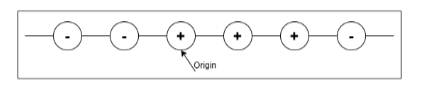
\includegraphics[width=0.5\linewidth]{drawio.png}
    \label{fig:enter-label}
\end{figure}


\begin{enumerate}
    \item[(a)] Find a feature map $\phi : \mathbb{R}^1 \to \mathbb{R}^2$ that maps the data in the original 1-D input space $x$ to a 2-D feature space $\phi(x) = (y_1, y_2)$ so that the data becomes linearly separable. Plot the dataset after mapping in the 2-D space. \hfill (8 points)
   
    we are given the following dataset in 1-D space:
    \[
    \text{Positive data points: } \{0, 1, 2\}, \quad \text{Negative data points: } \{-2, -1, 3\}.
    \]
    to transform the data into a linearly separable form, we can use the kernel function: polynomial kernel of degree 2:
    \[
    \phi(x) = (y_1, y_2) = (x, x^2).
    \]
    to transform the Positive data points:
    \\ the first positive data point is 0:
    \[
    \phi(0) = (0, 0^2) = \textbf{(0, 0)}
    \]
    the second positive data point is 1:
    \[
    \phi(1) = (1, 1^2) = \textbf{(1, 1)}
    \]
    the third positive data point is 2:
    \[
    \phi(2) = (2, 2^2) = \textbf{(2, 4)}
    \]
    to transform the Negative data points:
    \\ the first negative data point is -2:
    \[
    \phi(-2) = (-2, (-2)^2) = \textbf{(-2, 4)}
    \]
    the second negative data point is -1:
    \[
    \phi(-1) = (-1, (-1)^2) = \textbf{(-1, 1)}
    \]
    the third negative data point is 3:
    \[
    \phi(3) = (3, 3^2) = \textbf{(3, 9)}
    \]
    the transformed dataset in 2-D space is:
    \[
    \text{Positive data points: } \{(0, 0), (1, 1), (2, 4)\}, \quad \text{Negative data points: } \{(-2, 4), (-1, 1), (3, 9)\}.
    \]
    the plot of the dataset after mapping in the 2-D space is shown below:
   \(\textbf{Note: }\)  the figure might have floated to a different page.
    \begin{figure}[h!]
        \centering
        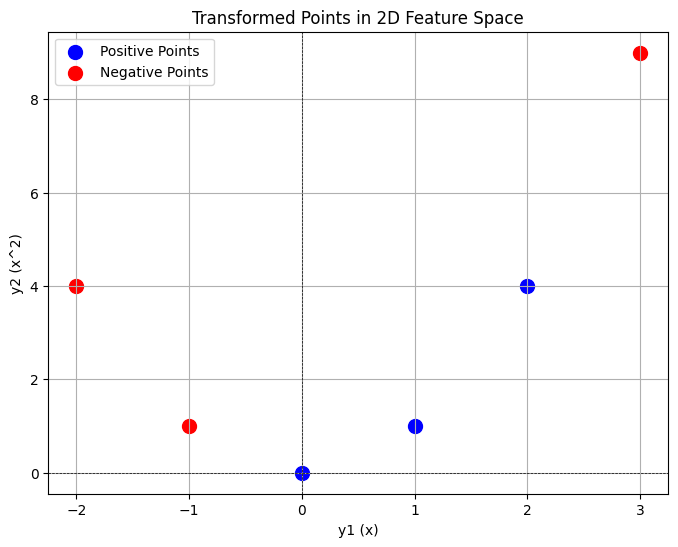
\includegraphics[width=0.5\linewidth]{2D_space.png}
    \label{fig:2D space}
    \end{figure}
    


    \item[(b)] Write down the equation for the separating hyperplane, 
    \(
    w_0 + w_1y_1 + w_2y_2 = 0
    \),
    given by a hard-margin linear SVM in the 2-D feature space. Draw this hyperplane on your plot and mark the corresponding support vector(s). \hfill (12 points)
    \\ the equation for the separating hyperplane is given by:
    \[
    w_0 + w_1y_1 + w_2y_2 = 0
    \]
    where the weights are given by:
    \[
    \mathbf{w} = \begin{bmatrix}
    w_0 \\
    w_1 \\
    w_2
    \end{bmatrix}
    \]
    the equation for the separating hyperplane is:
    \[
    w_0 + w_1y_1 + w_2y_2 = 0
    \]
    substituting the values of the weights:
    \[
    w_0 + w_1y_1 + w_2y_2 = 0
    \]
    \[
    w_0 + w_1x + w_2x^2 = 0
    \]
    \[
    w_0 + w_1x + w_2x^2 = 0
    \]
\end{enumerate}

\end{document}